\section{Объекты мышления: множества, предметы, отношения}
\begin{quotation}
  Мы слишком часто привыкли приписывать странное привычному. Я стараюсь вернуть знакомое в непривычное.

  - Рене Магритт
\end{quotation}
\subsection{Основные объекты: Множества и их элементы}
Математикам всегда приходится иметь дело с некоторыми объектами, которые под разными углами складываются в единое целое. Такие единицы называются множествами. Согласно Георгу Кантору, создателю теории множеств, множество - это "объединение определенных, хорошо дифференцированных объектов нашего восприятия или мышления в единое целое". Объекты, обобщенные таким образом, образуют элементы множества. Это основное определение того, что сегодня известно как "наивная теория множеств".

Современные математические теории говорят о множествах, между элементами которых существуют определенные отношения, определяемые базовыми понятиями, называемыми аксиомами. Именно это разнообразие возможных отношений между элементами множества приводит к разнообразию структурированных множеств, которые являются основной темой данной книги. Можно сказать, что именно эти отношения порождают самые разнообразные структуры. С другой стороны, множества без отношений между их элементами выглядят как аморфные сущности.

Особое достижение Кантора заключается в исследовании множеств с бесконечным числом элементов. С помощью своей "теории мощностей" он создал возможности для анализа в области бесконечности. (В этой главе, однако, мы ограничимся рассмотрением некоторых основ алгебры множеств).

Канторовское определение множества оказывается очень общим и выходит за рамки традиционных математических объектов - что вполне соответствовало духу изобретателя. Его "объекты для созерцания или размышления" включают в себя числа, зонтики и телевизоры, а также такие понятия, как свобода или избирательная тайна.

Однако сама широта концептуализации оказалась губительной. Если определение множества столь широко, то необходимо допустить и такие множества, как "множество всех абстрактных понятий" или даже "множество всех множеств", то есть множества, которые содержат сами себя. Это объясняется тем, что множество всех абстрактных понятий само является абстрактным понятием, а множество всех множеств само является множеством. Британский логик и философ Бертран Рассел показал, что такие общие концептуализации приводят к противоречиям (антиномиям). На самом деле достаточно спросить, содержит ли "множество всех множеств, не содержащих себя в качестве элемента" в понимании Рассела, себя в качестве элемента. Предположение, что это так, немедленно приводит к выводу, что оно не содержит себя в качестве элемента (потому что оно содержит именно те множества, которые не содержат себя в качестве элементов). С другой стороны, если предположить, что множество Рассела не содержит себя, то оно принадлежит множествам, которые обобщены в этом (Расселовском) множестве - следовательно, оно должно содержать себя как элемент. Независимо от ответа, вопрос о том, бреет ли себя цирюльник, который бреет всех, кто не бреется сам, приводит к противоречию.

Чтобы избежать подобных формулировок и вытекающих из них противоречий, базовые понятия и операции были заданы в системе строгих определений, которая получила название "аксиоматическая теория множеств" - в отличие от "наивной теории множеств" (аксиомы теории множеств также перечислены в главе об упорядоченных множествах). Для большинства математических целей вполне достаточно интерпретировать определение Кантора таким образом, что элементы множества должны быть определены еще до того, как они будут объединены в множество. Поскольку ни одно множество не содержит всего - не существует и всеобщего множества. Более философский подход: совокупность, которая содержала бы все объекты (множества) теории, сама не могла бы быть объектом теории. Поэтому определение элементов множества не должно сначала производиться самим множеством. Тогда исключаются множества, содержащие самих себя в качестве элементов, и больше нет места для противоречий.

Чтобы определить множество практически, у нас есть два способа: Либо мы перечисляем все его элементы, либо определяем множество по характерному свойству его элементов. Конечно, явное перечисление возможно только в том случае, если множество содержит конечное число элементов.

Несколько примеров проиллюстрируют эти возможности. Обозначения множеств даны заглавными латинскими буквами.

Также принято просто писать элементы рассматриваемого множества между фигурными скобками, например:

\vspace{0.5cm}
\(A = \{1,3,5,a,b,x,c\}\)
\vspace{0.5cm}

Вы также можете использовать просторечия для определения количества с помощью подходящего (однозначного) свойства:

\vspace{0.5cm}
B = Решения квадратного уравнения \(x^2+7x-1=0\)

X = буквы слова КАНТОР
\vspace{0.5cm}

Если x - элемент множества M, то мы пишем для него \(x \in M\).

Если x не принадлежит M, это выражается через \(x \notin M\)
\vspace{0.5cm}

Вот несколько примеров бесконечных множеств, где буквы представляют собой традиционные имена множеств с фиксированным значением:

\vspace{0.5cm}
\(\mathbb{N}\) = множество натуральных чисел \(\{1,3,5,\dots\}\)

\(\mathbb{N}_0\) = множество \(\mathbb{N}\) с нулевым значением \(\{0,1,2,\dots\}\)

F = \(\{3n + 5|n \in N_0\}=\{5,8,11,14,17,\dots\}\)
\vspace{0.5cm}

Читается: F равно множеству всех элементов вида 3n + 5, где n принадлежит множеству натуральных чисел (включая ноль).

\vspace{0.5cm}
\(\mathbb{Z}\) = множество целых чисел \(\{\dots,-2,-1,0,1,2,\dots\}=\{0,-1,1,-2,2,-3,3,\dots\}\)

\(\mathbb{Q}\) = множество рациональных чисел или дробей \(\{\frac{p}{q}|p,q \in \mathbb{Z},q \neq 0\}=\{\frac{p}{q}|p \in \mathbb{Z},q \in \mathbb{N}\}\)

I = \(\{x|x \in \mathbb{Q}, 0 \le x \le 1\}\)
\vspace{0.5cm}

В разговорной речи I также можно назвать множеством всех рациональных чисел x, удовлетворяющих неравенству \(0 \le x \le 1\).
Важно, чтобы оно было однозначным: должно быть ясно, является ли каждая мыслимая, возможная вещь элементом рассматриваемого множества или нет.

Используя обозначения \(S \subset T\) или \(S \subseteq T\), мы указываем, что множество S является подмножеством множества T, то есть каждый элемент \(s \in S\) также содержится в T: \(s \in T\). Эквивалентно, \(T \supset S\)(или \(T \supseteq S\)) означает, что T является надмножеством S и поэтому содержит это множество. (Я использую символы \(\subset\) и \(\subseteq\) равнозначно.) Из этого определения сразу следует, что каждое множество X содержит себя в качестве подмножества: \(X \subseteq X\) для каждого множества X.

Равенство множеств определяется следующим образом: Два множества равны тогда и только тогда, когда в них есть одинаковые элементы. Множества могут также выступать в качестве элементов других множеств, но, разумеется, всегда следует проводить точное различие между символами \(\in\) и \(\subset\) (или \(\subseteq\)); например:

\vspace{0.5cm}
\(M = \{a,b,c,\{1,2,3\}\}\) или также \(M = \{a,b,c,D\}\) с \(D=\{1,2,3\}\)
\vspace{0.5cm}

В этом случае:

\vspace{0.5cm}
\(\{1,2,3\}=D \in M\), а также \(a \in M\),

но

\(\{\{1,2,3\}\}=\{D\} \subset M\), а также \(a \subset M\).
\vspace{0.5cm}

По мере необходимости я буду вводить дополнительные обозначения.

\subsubsection{Много шума из ничего: Пустое множество}
Рассмотрим множество G целочисленных решений простого уравнения \(2x-1=0\).

Множество G однозначно определяется свойством его возможных элементов.
Решением уравнения является \(x=\frac{1}{2}\), но это не целочисленное решение.
Поэтому множество G не содержит ни одного элемента. Мы пишем \(G=\{\}\) или \(G=\emptyset\) и называем это множество пустым или нулевым.

Расширение понятия о множествах так же оправдано, как и введение нуля в числовой ряд.
Оно позволяет, как в нашем примере, определять множества, для которых заранее неизвестно, содержат они элементы или нет.
Таким образом, пустое множество существует, и оно однозначно.
Определение подмножества сразу же приводит к формальному утверждению: пустое множество является подмножеством любого множества.

\subsubsection{Диаграммы множеств и элементарные операции над множествами}
Для лучшей визуализации, множества часто представляют графически, используя диаграммы.
Однако эти диаграммы не выполняют никакой другой цели, кроме оказания мысленной помощи;
в частности, они не имеют доказательной силы. Представление множества \(M = \{a, b, c, D\}\) с \(D=\{1, 2, 3\}\) может выглядеть следующим образом:
\begin{center}
  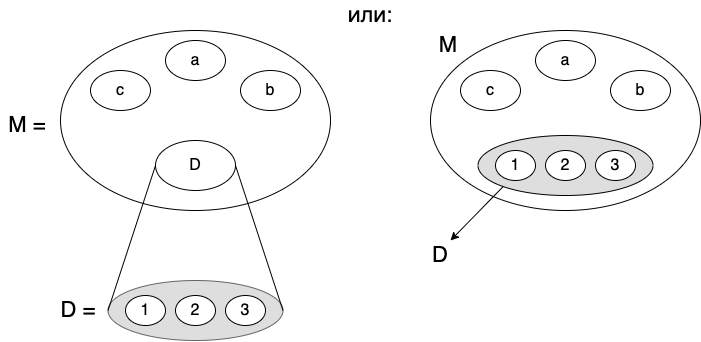
\includegraphics[scale=0.65]{001.png}
\end{center}
В частности, в формальных науках очень важны процессы, заключающиеся в получении из объектов последующих (подобных) объектов: например, последующие высказывания выводятся из существующих утверждений.
Аналогично, из существующих множеств образуются последующие множества.
Часто рассматриваемые случаи получения множеств - это форма объединения и усреднения.

Если есть два множества A и B, то объединение \(A \cup B\) определяется как множество элементов, которые принадлежат хотя бы одному из этих двух множеств.
При тех же условиях усреднение \(A \cap B\) определяется как множество элементов, которые принадлежат обоим множествам A и B.

Примечание: Среднее множество не имеет ничего общего со среднестатистическим или средним значением.
Также часто можно услышать о "пересечении".
\begin{center}
  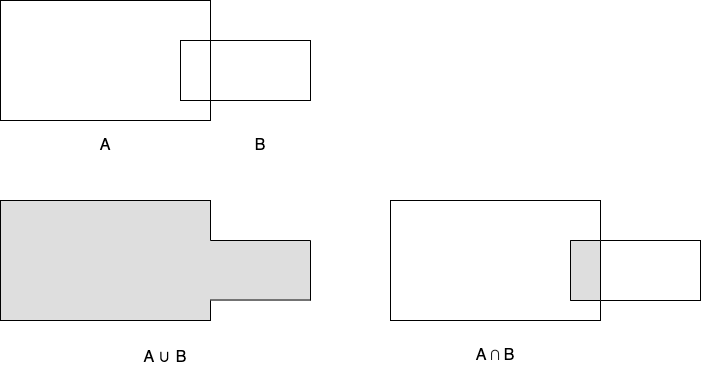
\includegraphics[scale=0.65]{002.png}
\end{center}
Недавно я прочитал литературную рецензию, в которой говорилось: "Этот автор обращается к сердцу всех доброжелателей и к уму всех глупцов.
Поскольку эти два сообщества образуют большой перекресток, вы можете ожидать высоких показателей продаж".

Два множества называются непересекающимися, если у них нет общего элемента, т.е. если их пересечение пусто.

Множество (простое) разностей \(A \setminus B\) между A и B - это множество всех элементов из A, которых нет в B:

\vspace{0.5cm}
\(A \setminus B = \{x \in A | x \notin B\}\)

\vspace{0.5cm}
Если M - подмножество X, то разностное множество \(X \setminus M\) называется дополняющим множеством M (относительно X) и обозначается \(M^c\).

Другой операцией над множеством является образование симметричной разности \(A \Delta B\), определяемой:

\vspace{0.5cm}
\(A \Delta B = (A \setminus B) \cup (B \setminus A)\)

\vspace{0.5cm}
Это множество всех элементов из объединения, которые не входят в усреднение (пересечение): \(A \Delta B = (A \cup B) \setminus (A \cap B)\). (Иногда это также называют булевой суммой множеств A и B).

\subsubsection{Декартово произведение}
Очень важным представлением множества является декартово произведение A × B двух множеств A и B: это множество всех упорядоченных пар (a, b), в которых первая компонента a является элементом A, а вторая компонента b - элементом B:

\vspace{0.5cm}
\(A \times B = \{(a,b) | a \in A, b \in B\}\)

\vspace{0.5cm}
Компоненты a и b упорядоченной пары также называются первой и второй координатами элемента \((a,b) \in A \times B\). Примеры:

Пусть: \(X=\{1,2,3\}, Y=\{a,b\}\)
\vspace{0.5cm}

Тогда

\(X \times Y=\{(1,a),(1,b),(2,a),(2,b),(3,a),(3,b)\},\)

\(Y \times X=\{(a,a),(a,b),(b,a),(b,b)\}.\)
\vspace{0.5cm}

Для бесконечных множеств X, Y декартовы произведения \(X \times Y, X \times X, Y \times X, Y \times Y\), разумеется, также бесконечны.
Например, декартово произведение множества \(\mathbb{R}\) вещественных чисел на само себя, \(\mathbb{R} \times \ \mathbb{R}\) или \(\mathbb{R}^2\) - это множество упорядоченных пар (x, y) с \(x \in \mathbb{R}\) и \(y \in \mathbb{R}\); соответственно, это и есть декартова плоскость (из "линейной алгебры и аналитической геометрии").
\begin{center}
  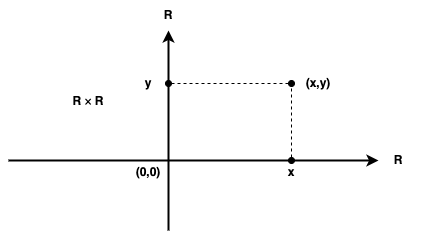
\includegraphics[scale=0.65]{003.png}
\end{center}
Термин "декартово произведение" становится понятным в связи с этим: Рене Декарт (Renatus Cartesius) основал аналитическую геометрию плоскости в первой половине XVII века, введя пары действительных чисел в качестве координат для точек плоскости.

Совершенно очевидная закономерность \((a,b)=(x,y)\) применима именно тогда, когда \(a=x\) и \(b=y\). Это равенство множеств можно легко распространить и на более чем два множества. Например: \(A=B=C=\{0,1\}\). Тогда декартово произведение \(A \times B \times C\) состоит из следующих упорядоченных троек, которые можно интерпретировать как координаты угловых точек (трехмерного) единичного куба:

\vspace{0.5cm}
\(\{(0,0,0),(0,1,0),(1,0,0),(1,1,0),(0,0,1),(0,1,1),(1,0,1),(1,1,1)\}\)

\vspace{0.5cm}
Формирование декартова произведения соответствующих множеств окажется незаменимым, особенно для так называемых производных функций (а также, например, для определения векторных пространств).

\subsubsection{Мощность, составляющая множество}
Возможности формирования дополнительных множеств из существующих практически неисчерпаемы.

Важным из них является формирование мощности множества \(P(X)\) существующего множества X; это не что иное, как множество всех подмножеств X:

\vspace{0.5cm}
\(P(X)=\{M|M \subseteq X\}\)

\vspace{0.5cm}

Для конечного множества с n элементами его мощность \(P(X)\) - составляет ровно \(2^n\) элементов (причем \(2^n > n\) всегда имеет место быть). Это легко показать методом доказательства "полной индукции".

Пример? Возьмем множество \(X=\{a,b,c\}\). Попробуем сформировать множество всех подмножеств X - мощность множества \(P(X)\). Для этого нам нужно учесть два действующих правила (о которых я уже говорил): Во-первых, пустое множество \(\{\}\) или \(G=\emptyset\) является подмножеством любого множества, а во-вторых, каждое множество всегда является подмножеством самого себя.

Лучший способ сформировать все подмножества X - действовать систематически: Сначала мы берем пустое множество: \(\{\}\); затем одноэлементные подмножества: \(\{a\}\), \(\{b\}\) и \(\{c\}\); затем двухэлементные подмножества: \(\{a,b\}\), \(\{a,c\}\), \(\{b,c\}\); и, наконец, трехэлементное подмножество - но это только само множество X: \(\{a,b,c\}\). В результате получается множество мощности:

\vspace{0.5cm}
\(P(X)=\{\emptyset, \{a\}, \{b\},\{c\},\{a,b\},\{a,c\},\{b,c\}, X\}\)

\vspace{0.5cm}

Таким образом, мы получаем в общей сложности 8 или \(2^3\) подмножества трехэлементного множества X, или иначе: множество мощности P (X) трехэлементного множества X состоит из \(2^3 = 8\) элементов. Рассуждения о подмножествах будут особенно важны в дальнейшем при определении топологических структур.

\subsubsection{Языковая традиция}
Если множество \(X \neq \emptyset\) ,то одним словом мы называем X непустым. Это традиция в математике, как и прилагательные - неевклидовы, некоммутативные и другие.
\pagebreak

\subsection{Соотношения: Отношения, отображения, связи}
Оглянувшись вокруг, мы обнаруживаем, что  множества повсюду: Множества домов, множества деревьев, множества листьев на деревьях, множества людей и так далее. А еще мы видим, что между множествами и между элементами множества могут существовать многочисленные отношения, иногда самые сложные сети отношений. Например, существует «теория о том, что любые два жителя Земли находятся не более чем в шести знакомствах друг от друга» - да, включая вас..... и меня. Но разве это максимальное число «шесть» не может быть значительно уменьшено, если мы также позволим книгам быть друзьями человека?

В этой главе представлены и описаны некоторые общие математические отношения между множествами и их элементами, а также их свойства.

Отношение - это особый способ связи элементов множества друг с другом. Например, дружба (между людьми) - это такое отношение, или принадлежность (между элементами и множествами, такими как \(3 \in N\)).
Но уравнение \(x + y =7\) также определяет отношение между «неизвестными» x и y.
В элементарной геометрии отношения между прямыми линиями или треугольниками определяются такими утверждениями, как g // h или \(\Delta ABC \sim \Delta A'B'C'\): Прямая g параллельна прямой h (//), один треугольник конгруэнтен другому \(\sim\).

В математике мы используем термин «отношение» и в других случаях. Например, мы говорим об отношении порядка между натуральными числами, которое описывается знаком < (меньше, чем): \(2 < 3\).
То, что мы будем определять как отношение, иногда более четко называется бинарным (двузначным) отношением. В случае трехзначного отношения это родительское отношение (Адам и Ева - родители Каина).
Однако у нас не будет возможности разобраться с трехзначными, четырехзначными или еще более сложными отношениями.

\subsubsection{Развитие математических объектов: общий взгляд}
Объекты современной математики возникли в результате многоступенчатого процесса абстрагирования, начавшегося с рассмотрения конкретных величин и отношений. Натуральные числа возникли, с одной стороны (и первоначально), в результате абстрактного процесса счета, а конкретные операции деления в повседневной жизни вскоре привели к появлению дробей или рациональных чисел.

Затем человек попытался выполнять такие операции счета и деления независимо от определенных, конкретных вещей, к которым он привычно применял эти операции, поскольку понял, что результаты его усилий не зависят от конкретных свойств исходных величин.
Он сформировал наборы чисел и расширил их: от натуральных чисел

\vspace{0.5cm}
\(\mathbb{N}=\{0,1,2,3,\dots\}\), к целым числам

\(\mathbb{Z}=\{0,-1,1,-2,2,-3,3,\dots\}\), к рациональным числам

\(\mathbb{Q}=\{\frac{a}{b}|a,b \in \mathbb{Z}, b \neq 0 ,\dots\}\),

\vspace{0.5cm}

перешел к действительным числам \(\mathbb{R}\) (которые также содержат иррациональные числа, такие как \(\sqrt {2}\) или длина окружности \(\pi\)) и, наконец, к комплексным числам \(\mathbb{C}\), которые могут быть представлены как упорядоченные пары действительных чисел:

\vspace{0.5cm}
\(\mathbb{C}=\mathbb{R} \times \mathbb{R} = \mathbb{R}^{2} = \{(x,y) | x,y \in \mathbb{R}\}\).

\vspace{0.5cm}

Одновременно изучались отношения между элементами этих числовых множеств, свойства определенных операций или связей между элементами и, наконец, (поэлементные) отображения между множествами чисел, причем эти отображения или демонстрации по сути сопоставимы с четко определенными ментальными ассоциациями.

Это была следующая ступень абстракции - она привела к появлению мира чисел, который и сегодня существует в человеческом сознании как самостоятельный мир, оторванный от исходных конкретных величин. Определенные связи или отношения, знакомые по конкретным вещам, были перенесены на числа. Это придало наборам чисел особые глобальные свойства - они преобразовали свою аморфную природу в структуры.

Наконец, следующим этапом абстрагирования стал отказ от особой природы чисел (как и множеств), поскольку было установлено, что отношения между множествами и между их элементами занимают все более важное место, поскольку эти отношения накладывают полезные и красивые структуры на все множества (а не только на множества чисел). (Схематично эти этапы показаны на странице 27. Эта иллюстрация примерно показывает многоступенчатый процесс абстрагирования, лежащий в основе развития математических объектов).

Конкретное и абстрактное все больше становились относительными понятиями. Таким образом, мир чисел, который уже представляет собой процесс абстракции, служит «конкретным» примером для еще более абстрактных величин и пространств на следующем уровне абстракции. Таким образом, каждый уровень дает конкретные примеры для следующего, более высокого абстрактного уровня.

\subsubsection{Отношения}
Мы еще не знаем с математической точностью, как определяется отношение между элементами x и y множества M. Но кажется правдоподобным, что каждое отношение должно однозначно определять множество всех тех
\begin{center}
  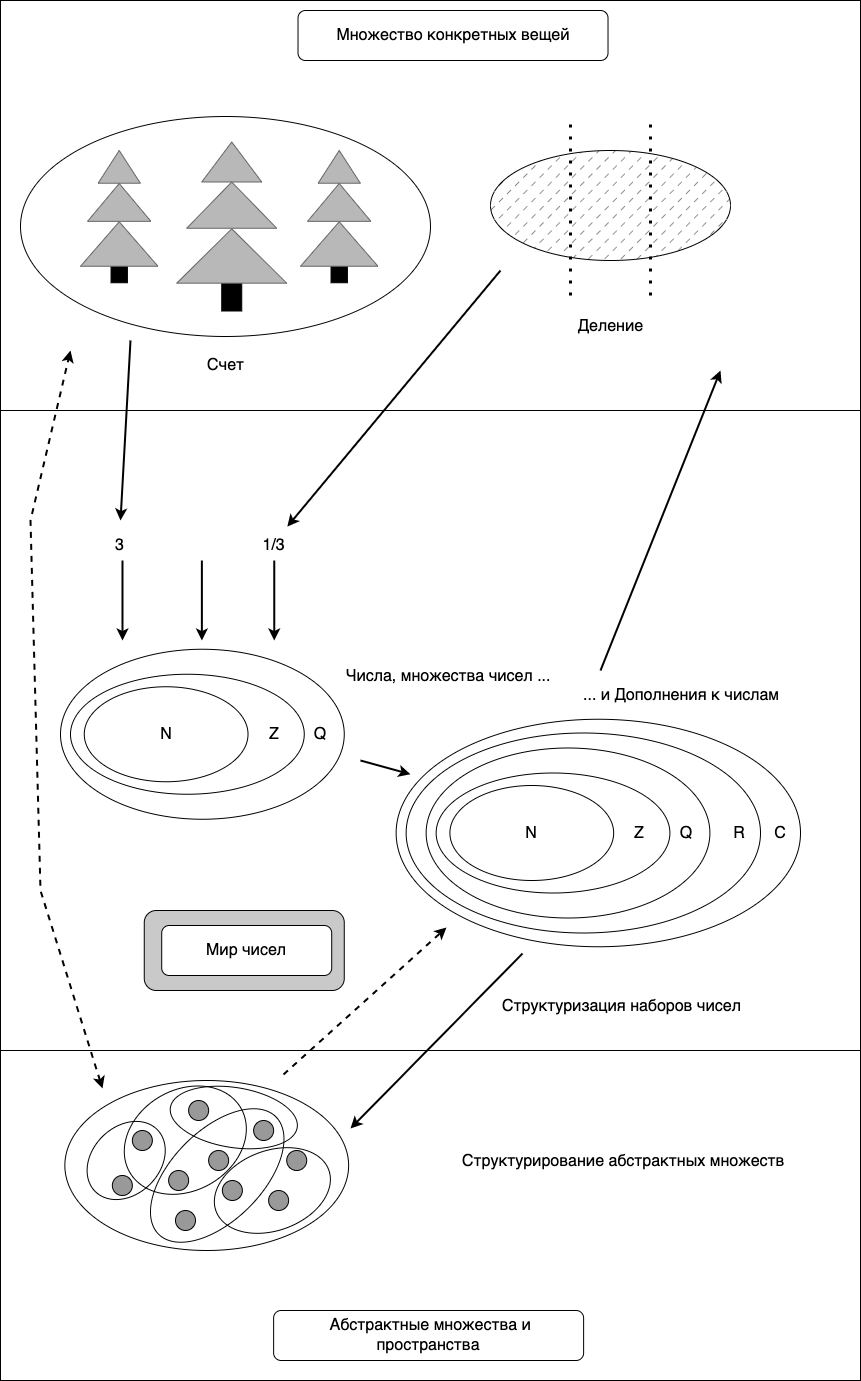
\includegraphics[scale=0.5]{004.png}
\end{center}
\pagebreak
упорядоченных пар \(x,y\), для которых первая координата x ко второй y просто находится в данном отношении. Если мы знаем отношение, мы знаем и множество, и, что еще лучше, если мы знаем множество, мы знаем и отношение.

Эти рассуждения устанавливают тесную связь между отношениями и множествами. Точная трактовка отношений использует эту эвристическую связь. Отношение просто определяется соответствующим множеством: отношение - это множество упорядоченных пар, и поэтому множество \(R\) является отношением, если каждый элемент \(R\) - упорядоченная пара, то есть если существование x и y при \(z =(x,y)\) всегда следует из \(z \in R\), где x и y - элементы множества \(M\).
Поскольку, с одной стороны, декартово произведение \(M \times M\) представляет собой множество всех упорядоченных пар элементов из \(M\), а с другой стороны, \(R\) представляет собой те упорядоченные пары, для которых первая координата находится в соответствующем отношении ко второй координате, \(R\) является лишь специальным подмножеством декартова произведения \(M \times M\):

\vspace{0.5cm}
\(R \subseteq M \times M\)

\vspace{0.5cm}

Если \(R\) - это отношение, то фактическое выражение \((x,y) \in R\) принято записывать также сокращенно \(xRy\) и говорить, как в разговорном языке, что \(x\) находится в отношении \(R\) к \(y\).

\subsubsection{Примеры}
Для следующих примеров знакомых отношений пусть \(M\) - это множество людей в городе. Обозначим элементы этого множества через \(a,b,c,\dots\). Конечно, это не означает, что у \(M\) не больше элементов, чем алфавит; нам нужно всего несколько букв для описания.

(1) Между некоторыми элементами \(M\). существуют отношения "отец-ребенок":

а V b: a отец для b.

Для полного описания этого отношения в \(M\) можно перечислить все пары отец-ребенок  \((a,b) \in V \subset M \times M\).

(2) Между некоторыми элементами \(M\) существуют родственные отношения:

\(sGt\): s и t - родные братья и сестры.

Но, конечно, возможны не только семейные отношения.

(3) Отношение лексикографического порядка. Мы упорядочиваем элементы M в алфавитном порядке в соответствии с их названием. Майер стоит перед Мейером, а Шмидт, Франц, перед Шмидтом, Георгом.

\(a \lhd b\) (читается: a перед b): a идет в алфавитном порядке перед b.

\subsubsection{Другие знакомые примеры}
Принадлежность к одной и той же профессиональной группе иногда является значимым отношением: a L b (a и b - являются учителями).

Мы могли бы распределить жителей нашего города по возрасту, росту или весу. Поскольку люди покупают и продают в городе, мы также можем рассмотреть деловое отношение a K b (a является клиентом b).
В каждом множестве X каждый элемент x \(\in\) X тождественен самому себе. Это отношение известно как отношение тождества или равенства;

\vspace{0.5cm}
\(\Delta = \{(x,x)|x \in X\} \subset X \times X\)

\vspace{0.5cm}

Наименьшим отношением в X является пустое множество \(\emptyset\), а наибольшим - декартово произведение \(X \times X\).

\subsubsection{Свойства отношений}
Отношения обладают определенными свойствами, и полезно дать им название. Ниже приведены общепринятые обозначения:

Отношение \(R\) в множестве \(M\) называется
\begin{itemize}
  \item транзитивным, если из \(aRb\) и \(bRc\) всегда следует \(aRc\),
  \item рефлексивным, если \(aRa\) действителен для всех \(a \in M\),
  \item антирефлексивным, если \(aRa\) не распространяется ни на один элемент множества,
  \item симметричным, если из \(aRb\) всегда получается \(bRa\),
  \item асимметричным, если \(aRb\) всегда исключает \(bRa\),
  \item антисимметричным, если из \(aRb\) и \(bRc\) всегда следует \(a=b\).
\end{itemize}

Отношения < (меньше, чем) или ≤ (меньше или равно), а также отношение лексикографического порядка \(\angle\) являются переходными;
то же самое относится и к отношению "быть родственником".
Однако дружеские отношения не обязательно являются транзитивными: если a и b - друзья, а b и c - тоже друзья, из этого не обязательно следует, что a и c - друзья;
они даже не обязательно должны знать друг друга или могут быть врагами.

Отношения между братьями и сестрами рефлексивны, если мы согласны, что \(sGs\) должно быть всегда (т. е.
что каждый является своим братом или сестрой). Отношение равенства или тождества = также рефлексивно, потому что \(x=x\) всегда применимо.

Отношение "отец - ребенок", несомненно, антирефлексивно, как и отношение < (меньше, чем), поскольку \(x < x\) не относится ни к одному x.

Отношения между братом и сестрой и отношения принадлежности к одной профессиональной группе являются симметричными.

Отношения между отцом и ребенком, несомненно, асимметричны. Асимметричные отношения всегда также антирефлексивны (хотя обратное не обязательно верно).

Конечно, существуют отношения, которые не обладают ни одним из описанных свойств.

\subsubsection{Порядки и эквиваленты}
Существует два типа отношений, которые важны для всей математики и обозначаются следующим образом:
\begin{enumerate}
  \item Отношение, которое является асимметричным и транзитивным, называется (строгим) отношением порядка или, сокращенно, порядком.
  \item Отношение, которое является рефлексивным, симметричным и транзитивным, называется отношением эквивалентности, или эквивалентностью, для краткости.
  \end{enumerate}

Очевидно, что и лексикографический порядок \(\angle\), и отношение \(<\) (меньше, чем) в множестве натуральных (или вещественных) чисел являются отношениями порядка.
С другой стороны, отношение родства G, параллельность // (между прямыми), конгруэнтность (между треугольниками) и отношение равенства или тождества являются эквивалентностями.

\subsection{Отображения, Функции}
Со времен основания исчисления Исааком Ньютоном и Готфридом Вильгельмом Лейбницем понятие функции играет важную роль в математических описаниях.
В механике, например, движения точки массы описываются функциями, которые мысленно приписывают время \(t\) местоположению точки массы, описываемому координатами \(x, y, z\).

Динамика изменения температуры \(T\) в точке пространства также является функцией времени, которая присваивает определенную температуру \(T\) для точки пространства в каждый момент времени \(t\).
Температурная кривая - это графическое представление такого изменения температуры в точке пространства с течением времени.

Таким образом, функция имеет характер отношения - связи - между величинами (пространственными точками, температурами, точками времени или интервалами).
И действительно, понятие функции можно определить как особое отношение (как станет ясно из "второго определения" ниже).

Однако математика воздерживается от специальных множеств и элементов и использует терминологию теории множеств для определения функции, чтобы прийти к гораздо более общей концепции:

\subsubsection{Первичное определение}
\(X\) и \(Y\) - наблюдаемые множества.
Величина \(f\), которая каждому элементу \(x \in X\) ставит в соответствие ровно один элемент \(y \in Y\), в форме выражения \(x \rightarrow y = f(x)\), называется \textit{функцией} или \textit{отображением} из \(X\) в \(Y\), в форме \(f:X \rightarrow Y\).

\subsubsection{Примечания и примеры}
Не бойтесь символически - сокращенных - обозначений \(x \rightarrow y =f(x)\) (поэлементное определение) и \(f: X \rightarrow Y\) (количественное представление присваивания).

Элемент \(y = f(x)\) называется значением (функции), которое функция \(f\) принимает в позиции (аргумента) \(x\); эквивалентно можно также сказать, что функция \(f\) отображает элемент  \(x\) в элемент или преобразует \(x\) в \(y\), или что элемент y однозначно присваивается элементу \(x\) функцией \(f\).
Соответственно, термины отображение, преобразование, присвоение, оператор (и другие) иногда используются как синонимы функции.
Большинство математиков считают аргументно-значное описание функции более прозрачным, чем любое другое.

Конкретное функциональное выражение всегда определяется элемент за элементом;
например, отношение \(x+y=7\) между неизвестными x и y определяет функцию между (натуральными, рациональными или вещественными) числами ( \(\mathbb{N} \rightarrow \mathbb{N}\), \(\mathbb{Q} \rightarrow \mathbb{Q}\) или \(\mathbb{R} \rightarrow \mathbb{R}\)), поскольку можно решить уравнение \(y=7-x\) и таким образом получить однозначное соответствие \(x \rightarrow y = 7-x\), которое определено для всех рассматриваемых чисел x.

Иллюстрацией может послужить и распределение гражданин \(\rightarrow\) удостоверение личности, если мы предположим, что каждый (совершеннолетний) гражданин современного конституционного государства имеет удостоверение личности.

Внимательный читатель уже давно понял, что с точки зрения математики отображение - это не иллюстрация факта, как иллюстрация в книге. Еще раз: (математическое) отображение \(f\) из множества \(X\) в множество \(Y\) - это уникальное соответствие между элементами \(X\) и \(Y\), которое ставит каждый элемент \(X\) в соответствие ровно одному элементу \(Y\).

\(X\) - область определения, а \(Y\) - область выбора значений или отображения. Множество всех элементов в \(Y\), определяемое отображением, называется отображением \(X\) (при задании отображения \(f\)) и обозначается \(f[X]\).
Поскольку конкретные отображения определяются элемент за элементом, термин " отображение" также применяется к соответствующим элементам. Разумеется, все только предполагается: как множества \(X\) и \(Y\) вместе с их элементами, так и само уникальное соответствие или отображение (или функция).
